\documentclass
[rmp,reprint,
twocolumn,amsmath,showkeys,letterpaper,raggedbottom]{revtex4-2}
\usepackage{times}
\usepackage[bookmarks=false]{hyperref}
\usepackage{graphicx}
\usepackage{draftwatermark}
\def\thesection{\arabic{section}}
\def\thetable{\arabic{table}}
\bibliographystyle{preprint}
\def\figuredir{.}

\begin{document}

\title{Sensor trajectory estimation by triangulating LIDAR returns}
\date{\today}
\author{Charles F. F. Karney}
\email{charles.karney@sri.com}
\affiliation{\href{http://www.sri.com}{SRI International},
201 Washington Rd, Princeton, NJ 08543-6449, USA}

\begin{abstract}

The paper describes how to recover the sensor trajectory for an aerial
lidar collect using the data for multiple-return lidar pulses.  This
work extends the work of \citet{gatziolis19} by performing a
least-squares fit for multiple pulses simultaneously with a spline fit
for the sensor trajectory.  The paper also shows how to incorporate
scan-angle data following the method of \citet{hartzell20}.

\end{abstract}

\maketitle

\section{Introduction}\label{intro}

Lidar data sets, typically provided in the form of ``{\tt las}'' files
\citep{las}, often do not contain information on the location of the
sensor platform as a function of time.  For datasets which include the
GPS time for each return, it is possible to identify the multiple
returns originating from a given lidar pulse and thus determine its
direction.  By combining the data for multiple pulses emitted in a short
time, it is possible to ``triangulate'' for the position of the sensor.
This idea was proposed by \citet{gatziolis19} who showed how to obtain a
full sensor trajectory.

Here we reformulate this problem with a view to obtaining a more
accurate trajectory.  The trajectory is modeled as a cubic spline fit.
Such a fit independently fits the $x$, $y$, and $z$ components
of $\mathbf R(t)$.  The {\it unknowns} in this model are the parameters
specifying the cubic splines.  The {\it knowns} are the positions (and
times) of the multiple returns from individual lidar pulses.  The
optimization problem is then to adjust parameters specifying the
trajectory to minimize the RMS error between the returns and a ray
drawn from the sensor position to the mean position of the return.
This is a rather complex nonlinear optimization problem.  Fortunately,
it is one that is easily handled by the software library \citet{ceres}.

The errors in this problem are primarily quantization errors in the
positions of the returns.  In the normal post-processing of a lidar
collect, the positions of the returns are computed from IMU data from
the sensor platform, the scan angle of the lidar sweep, and timing
information for the returns.  If these positions were recorded
accurately, it would be possible to determine a precise ray for a given
pulse (with 2 or more returns) and sensor position could be accurately
triangulated from the rays nearly simultaneous pulses.  However, the
default precision of the return positions in a {\tt las} file is
$0.01\,\text{m}$.  If the two returns are $2\,\text{m}$ apart and the
sensor is flying $1000\,\text{m}$ above the ground then, then the
possible rays consistent with the return data span $5\,\text{m}$ at the
altitude of the sensor.  The uncertainty in the triangulation with such
rays is increased because of ill conditioned triangles (leading chiefly
to a large uncertainty in the height of the sensor).

\section{Fixed sensor}

In order to introduce the concepts, let us start first by assuming
that the sensor is fixed and emits $n$ multi-return pulses, indexed
by $i \in [1,n]$.  We shall only consider the first and last returns
(ignoring any intermediate returns).  We denote positions of the
returns by
\begin{equation} \label{return}
 \mathbf r_i^\pm = \mathbf r_i \pm d_i \mathbf p_i,
\end{equation}
where superscripts $\pm$ denote first and last returns, $\mathbf
p_i$ is the unit vector in the direction from the last to the first
return, and $d_i$ is half the distance between the returns.

\subsection{The reverse method}

The goal now is to determine the position $\mathbf R$ consistent
with these returns.  One approach is to consider the $n$ rays
\begin{equation}
 \mathbf r_i + s_i \mathbf p_i
\end{equation}
where the distance along the ray is parameterized by $s_i$ and to
solve the $3n$ equations
\begin{equation}
 \mathbf r_i + s_i \mathbf p_i - \mathbf R = \mathbf h_i \approx 0
\end{equation}
for the $3+n$ unknowns $\mathbf R$ and $s_i$.  This is an overdetermined
system for 2 or more pulses and then we can use standard linear algebra
methods to find the best solution which minimizes $\sum_i h_i^2$, the
so-called least-squares solution.

This is the approach used by \citet{gatziolis19} who consider just pairs
of pulses $n = 2$.  The problem is that the resulting solution for
$\mathbf R$ is typically not the optimal solution for the trajectory
problem because the system of equations does not involve the return
separation $d_i$ so pulses with closely separated returns and treated
equally to pulses with widely separated returns.  In reality, the latter
returns should be weighted more heavily.

Gatziolis and McGaughey address this problem by selecting an {\it optimal}
pair of returns based on the return separation and the angle between
the pulses.  This is based on a weighting function which needs to be
separately estimated.

We use a simplified version of this linear least-squares problem to
find an initial trajectory for our method described below.  We use the
$z$ component of the residue equations to eliminate $s_i$ from the
system.  The equations are then
\begin{align*}
\biggl( r_{i,x} - \frac{p_{i,x}}{p_{i,z}} r_{i,z} \biggr) -
\biggl( R_x - \frac{p_{i,x}}{p_{i,z}} R_z \biggr) = h_{i,x} \approx 0, \\
\biggl( r_{i,y} - \frac{p_{i,y}}{p_{i,z}} r_{i,z} \biggr) -
\biggl( R_y - \frac{p_{i,y}}{p_{i,z}} R_z \biggr) = h_{i,y} \approx 0.
\end{align*}
We can write this as the explicit overdetermined linear system
\begin{equation}
\mathsf A \cdot \mathbf R - \mathbf B = \mathbf H \approx 0,
\end{equation}
where $\mathsf A$ is the $2n \times 3$ matrix
\begin{equation}
\mathsf A = \begin{pmatrix}
\vdots & \vdots & \vdots \\
1 & 0 & - p_{i,x}/p_{i,z} \\
0 & 1 & - p_{i,y}/p_{i,z} \\
\vdots & \vdots & \vdots
\end{pmatrix}
\end{equation}
(two rows for each of the $n$ pulses), $\mathbf B$ is the $2n$
column vector
\begin{equation}
\mathbf B = \begin{pmatrix}
\vdots \\
r_{i,x} - (p_{i,x}/p_{i,z}) r_{i,z} \\
r_{i,y} - (p_{i,y}/p_{i,z}) r_{i,z} \\
\vdots
\end{pmatrix},
\end{equation}
and $\mathbf R$ is the unknown sensor position to solve for.

This reduces the problem to $2n$ equations for $3$ unknowns.  In this
formulation we determine the horizontal plane $z = R_z$ in which the
rays are most tightly clustered.  This is {\it not} the same problem as
before; however with typical aerial lidar collects the two solutions for
$\mathbf R$ will be reasonably close.  The difference is immaterial in
our application since this solution for $\mathbf R$ is only used as an
initial estimate.

It's also possible to extend this method to allow the position of the
sensor to be a function of time, for example,
\begin{equation*}
  \mathbf R = \mathbf R_0 + \mathbf V t.
\end{equation*}
The least-squares problem is now
\begin{equation}\label{lsprob}
\mathsf A \cdot
\begin{pmatrix}
  \mathbf R_0\\
  \mathbf V
\end{pmatrix}
- \mathbf B = \mathbf H \approx 0,
\end{equation}
where $\mathsf A$ is now the $2n \times 6$ matrix
\begin{equation}
\mathsf A = \begin{pmatrix}
\vdots & \vdots & \vdots & \vdots & \vdots & \vdots \\
1 & 0 & - p_{i,x}/p_{i,z} & t_i & 0   & - t_i p_{i,x}/p_{i,z} \\
0 & 1 & - p_{i,y}/p_{i,z} & 0   & t_i & - t_i p_{i,y}/p_{i,z}\\
\vdots & \vdots & \vdots & \vdots & \vdots & \vdots
\end{pmatrix}
\end{equation}
(and $\mathbf B$ is unchanged).  Here $t_i$ is the time of the $i$th
pulse.

Because pulses with widely separated returns constrain the possible
position of the sensor more strongly than those with nearby returns, we
multiply the rows in $\mathsf A$ and $\mathbf B$ associated with the
$i$th pulse by $d_i$, thereby appropriately {\it weighting} the
least-squares problem.

As a practical matter, Eq.~(\ref{lsprob}) can be solved to give $\mathbf
R_0$ and $\mathbf V$ by a suitable linear algebra package.  For example,
its solution can be obtained using \citet{eigen} with, for example,
\begin{equation*}
\text{\tt RV = A.jacobiSvd().solve(B);}
\end{equation*}

\subsection{The forward method}

We term the above method of estimating $\mathbf R$ described above the
{\it reverse} method, because the rays are traced back from the returns
to the sensor.  An alternative is to trace the rays from $\mathbf R$ to
the midpoint of returns, the {\it forward} method.  Thus each ray is
given by
\begin{equation} \label{pulse}
 \mathbf r_i + s_i \hat{\mathbf q_i},
\end{equation}
where $\mathbf q_i = \mathbf R - \mathbf r_i$.  The rays now all
intersect at $\mathbf R$ and the optimization problem is to find
$\mathbf R$ and $s_i$ such that Eq.~(\ref{pulse}) is approximately equal
to the position of the first return, $\mathbf r^+$, from
Eq.~(\ref{return}), i.e.,
\begin{equation}
  d_i \mathbf p_i - s_i \hat{\mathbf q_i} = \mathbf e_i \approx 0.
\end{equation}
Again we have $3n$ equations with $3 + n$ unknowns.  However the
quantities that are being minimized, $\mathbf e_i$, is the distance
between the ray and the given positions of the returns.  This method
now naturally gives more weight to widely separated returns and the
solution will similarly be more heavily governed by rays forming
well-conditioned triangles.

Incidentally, the ray from $\mathbf R$ to $\mathbf r_i$ passes equally
close to the first and last returns, so it is only necessary to the
minimize the distance to the first returns.

This system of equations is no longer linear, so it cannot be solved by
linear algebra techniques.  However, it is ideally suited for the Ceres
Solver package.  This finds the least-squares solution for nonlinear
optimization problems.  It also features
\begin{itemize}
\item
  Automatic determination of the Jacobian needed to find the solutions.
  This is achieved by writing the formulas in standard notation but with
  the variables having a C++ type ``Jet'' which combines a quantity and
  its derivative and, through overloaded operators and functions,
  follows all the standard rules of differentiation.
\item
  A robust optimization.  A standard problem of least-squares methods is
  that outliers in the data can skew the solution away from the
  ``right'' one.  Ceres Solver includes a variety of ``loss functions''
  which cause the effect of errors in the equations to fall off past
  some threshold.  For example in this case, the threshold for the loss
  functions might be set to $0.01\,\text{m}$.
\end{itemize}

\subsection{Simplifying the forward method}

We can simplify the problem by observing that $\mathbf e_i$ is minimized
with $s_i \approx d_i$ and that the resulting $\mathbf e_i$ then spans a
two-dimensional space perpendicular to $\mathbf p_i$.  Thus we can
approximate the error $\mathbf e_i$ by projecting the $\mathbf R -
\mathbf r_i$ onto the plane perpendicular to $\mathbf p_i$ at the first
return.  The first step is to convert to a primed coordinate system with
$\mathbf r_i$ at the origin and with the $\mathbf z'$ axis parallel to
$\mathbf p_i$.  This is achieved by the rotation matrix
\begin{equation}
 \mathsf M_i = \begin{pmatrix}
\displaystyle
\frac{p_{i,x}^2 p_{i,z} + p_{i,y}^2}{p_{i,x}^2+p_{i,y}^2} &
\displaystyle
\frac{-(1 - p_{i,z}) p_{i,x} p_{i,y}}{p_{i,x}^2+p_{i,y}^2} &
-p_{i,x} \\[1ex]
\displaystyle
\frac{-(1 - p_{i,z}) p_{i,x} p_{i,y}}{p_{i,x}^2+p_{i,y}^2} &
\displaystyle
\frac{p_{i,x}^2 + p_{i,y}^2 p_{i,z}}{p_{i,x}^2+p_{i,y}^2} &
-p_{i,y} \\[1ex]
p_{i,x} & p_{i,y} & p_{i,z}
\end{pmatrix}.
\end{equation}
This matrix rotates the coordinate system about the axis $\mathbf z
\times \mathbf p_i$.  Applying this translation and rotation to the
sensor position gives
\begin{equation}
 \mathbf q'_i = \mathsf M_i \cdot \mathbf q_i
\end{equation}
Finally we project $\mathbf q'_i$ onto the plane $z' = d$ which gives
\begin{equation}
\mathbf e'_i = \frac{d_i}{q'_{i,z}}
\begin{pmatrix}
q'_{i,x}\\[1ex]
q'_{i,y}
\end{pmatrix}.
\end{equation}
Now the number of unknowns is just $3$, the coordinates of $\mathbf
R$, and the number of equations is $2n$, $\mathbf e_i \approx 0$
for each two-component vector $\mathbf e_i$

Solving this least-squares problem with Ceres Solver entails writing a
C++ class implementing a ``residue block''.  The constructor for the
class takes the {\it knowns} for a particular pulse, i.e., $\mathbf
r_i$, $\mathbf p_i$, and $d_i$, and implements a function object
which accepts the {\it unknowns} $\mathbf R$ as input and returns the
residue $\mathbf e_i$.  This entails merely expressing the equations
above as computer code.  The problem is specified by $n$ such
residue blocks and an initial guess for $\mathbf R$ (obtained, for
example, by the reverse linear least-squares problem).  Ceres Solver
repeatedly invokes the function objects while adjusting $\mathbf R$
to minimize $\sum e_i^2$.  Because of the automatic differentiation
built into Ceres Solver, it can compute the Jacobian for the problem
which says how each component of $\mathbf e_i$ changes as each
component of $\mathbf R$ is varied.  This allows Ceres Solver to
vary $\mathbf R$ in an optimal way in its search for the
least-squares solution.

\section{The trajectory computation}

The discussion above solves for the sensor position at a single instant
of time.  Of course, the sensor position is typically moving and it is
convenient to model the motion as a cubic spline.  One approach would be
to perform a series of fixed sensor calculations, e.g., at
$0.01\,\text s$ intervals including for each calculation 10 pulses
sampled at $0.001\,\text s$ intervals and then to fit a spline to
the resulting positions.

This approach has the drawback that some of the positions may be better
approximated than others and the spline fit should respect this.  This
could be achieved by assigning weights to the various position estimated
and this, essentially, is how Gatziolis and McGaughey addressed this
issue.  However this put another layer of complexity into the problem.

However, in the spirit of Ceres Solver, it make more sense to pose the
entire exercise as a single least-squares problem.  Let's start by
describing how to express a cubic spline.

\subsection{The cubic spline}

A cubic spline is a piece-wise cubic polynomial function which in our
application we will use to approximate $\mathbf R(t)$.  Each component
of $\mathbf R(t)$ can be fit independently of the others.  So we only
need to consider a cubic spline for a scalar function $f(t)$ defined
between $T_0$ and $T_K = T_0 + K \,\Delta t$.  The time interval divided
in $K$ blocks of duration $\Delta t$, with the $k\text{th}$ block
consisting of the interval $T_k \le t < T_{k+1}$ where $T_k = T_0 + k
\,\Delta t$ and $k \in [0,K)$.  At internal block boundaries, $t = T_k$
for $k \in (0, K)$, we require that $f(t)$, $f'(t)$, and $f''(t)$ be
continuous.

We shall specify the cubic polynomial for the $k\text{th}$ block
by the values of $f(t)$ and $g(t) = \Delta t\,f'(t)$ at the block
boundaries.  It is convenient to introduce a scaled centered time
variable the block $\tau = (t - T_k)/\Delta t - \frac12$.  At the
block boundaries, we have $f = f_k$ and $g = g_k$ at $\tau =
-\frac12$ and $f = f_{k+1}$ and $g = g_{k+1}$ at $\tau =
\frac12$.  It is now a simple matter, e.g., by using the algebra
system, \citet{maxima}, to find the polynomial satisfying the boundary
conditions
\begin{equation}
f(\tau) = a_0 + a_1 \tau + a_2 \tau^2 + a_3 \tau^3,
\end{equation}
where
\begin{align*}
 a_0 &= \textstyle\frac18 (4 f_+ - g_-),\\
 a_1 &= \textstyle\frac14 (6 f_- - g_+),\\
 a_2 &= \textstyle\frac12 g_-,\\
 a_3 &= -2 f_- + g_+,\\
 f_\pm &= f_{k+1} \pm f_k, \\
 g_\pm &= g_{k+1} \pm g_k.
\end{align*}

By specifying the cubic polynomial by its values and derivatives at
the block boundaries, we ensure continuity of $f(t)$ and $f'(t)$.
The jump in the second derivative is given by
\begin{equation}
  \Delta f''(T_k) =
  \frac{6 (f_{k+1}-f_{k-1}) - 2 (g_{k+1}+g_{k-1}) - 8 g_k}
       {\Delta t^2}.
\end{equation}
We will then add $\Delta f''(T_k) \approx 0$ to the optimization problem.

In some situations, portions of a lidar collect might consist of ``only
returns''.  These are, of course, not useful of determining the sensor
trajectory by this method.  However, if the stretch of only returns
spans multiple blocks in the cubic spline, then the spline determination
becomes badly conditioned.  We address this by enforcing an {\it
  additional} constraint on the boundaries between two block with few
multiple returns, namely that the third derivative is continuous.  The
jump in the third derivative is
\begin{equation}
  \Delta f'''(T_k) =
  \frac{4f_k - 2(f_{k+1}+f_{k-1}) + (g_{k+1}-g_{k-1})}
       {\Delta t^3}.
\end{equation}
In order to improve the smoothness of the trajectory, we add a
constraint $\Delta f'''(T_k) \approx 0$ for all block boundaries.
However, the weight for this constraint is very small except when the
boundary separates blocks essentially devoid of multiple returns.

\subsection{The optimization problem}

We are now ready to set up the optimization problem for the entire
trajectory.  The knowns are $t_i$, $\mathbf r_i$, $\mathbf p_i$, and
$d_i$ for $n$ pulses.  These are the same as for the fixed sensor
problem with the addition of the time $t_i$ for each pulse.  The
unknowns are the sensor positions, $\mathbf R(t)$ and velocities,
$\mathbf R'(t)$, at the block boundaries $t = T_k$ for $k \in [0,K]$.

The residue block for Ceres Solver now includes the time $t_i$.  Each
pulse is assigned to a particular time block and the constructor
converts this time to the scaled time $\tau$.  The corresponding
function object now takes the trajectory position and velocities at the
block boundaries as input.  It then uses the stored value of $\tau$ to
evaluate the corresponding cubic polynomials for the 3 components of the
sensor position $\mathbf R(t_i)$.  The calculation then proceeds as in
the fixed-sensor case and returns a two-component vector for the
residue.

There is now also a new type of residue block to enforce the continuity
of the acceleration at the internal block boundaries.  The function
object takes $\mathbf R(T_{k\pm1})$, $\mathbf R'(T_{k\pm1})$, and
$\mathbf R'(T_k)$, and returns the jump in $\mathbf R''(T_k)$.

Overall there are $6(K+1)$ unknowns (the positions and velocities at the
block boundaries).  The number of equations is $2n$ for the pulse
residues, plus $3(K-1)$ for the acceleration jump constraints, plus,
optionally, another $3(K-1)$ for the constraints on the jump in the
third derivatives.

\begin{figure*}[tb]
\begin{center}
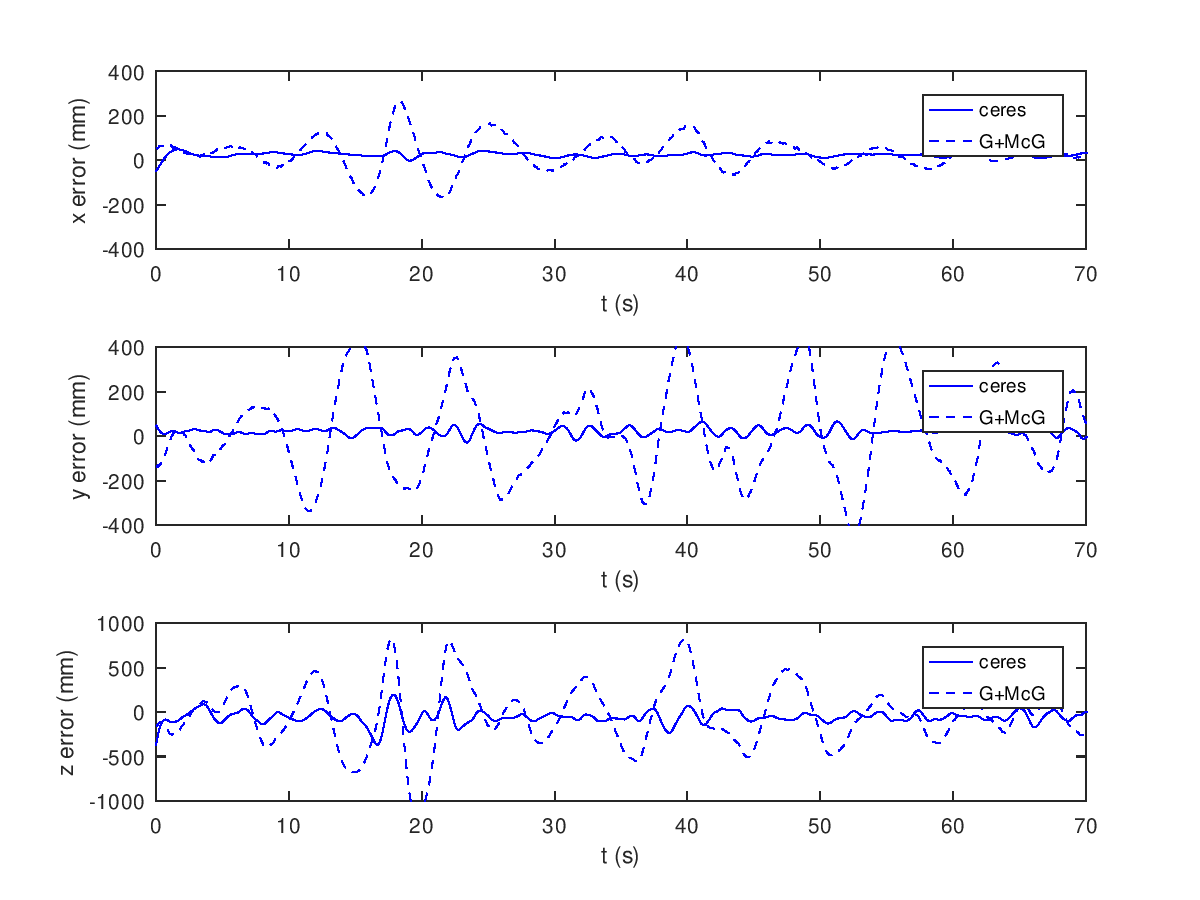
\includegraphics[scale=0.75,angle=0]{\figuredir/uh0}
\end{center}
\caption{\label{test} The discrepancy in the estimated trajectory from
  the IMU data for the sensor for a lidar capture over Houston, TX, the
  curves labeled ``ceres.''  The RMS error in the horizontal,
  resp.~vertical, position of the sensor is $36\,\text{mm}$,
  resp.~$90\,\text{mm}$.  For comparison, also shown is the discrepancy
  using the method of \citet{gatziolis19}, the curves labeled ``G +
  McG'', with corresponding horizontal, resp.~vertical, errors of
  $221\,\text{mm}$, resp.~$354\,\text{mm}$.}
\end{figure*}

\section{Testing}

We have tested this on flights lasting about a minute with $\Delta t
= 1\,\text s$ and sampling one multi-return pulse every
$0.001\,\text s$ from the lidar data (we select the pulse with the
largest distance between its first and last returns).  Even though
this involves a system of tens of thousands of equations, Ceres Solver
handles it without difficulty in a few seconds of CPU time.

Figure \ref{test} shows the discrepancy in the estimated trajectory from
the IMU data for the sensor for a lidar capture over Houston, TX.

\section{Including the scan angle data}

The method outlined above depends on there being sufficient multiple
returns present in the data.  \citet{hartzell20} suggested using the
{\it scan angle} of the lidar pulse as an alternative method for
triangulating the position of the sensor platform.  This data can be
seamlessly merged into our method allowing the sensor position to be
estimated even in the absence of multiple returns.  This has the added
benefit that the attitude of the sensor platform can be estimated.

The scan angle of the lidar pulse is the angle measured rightwards from
nadir of the lidar pulse as it sweeps left and right either side of the
sensor platform.  In some {\tt las} formats, this is only recorded
to the nearest whole degree.

We start by determining the direction of the laser pulse given the yaw
$\psi$, pitch $\theta$, and roll $\phi$ of the sensor platform and the
scan angle $\alpha$.  The standard coordinate system is $x$ east, $y$
north, and $z$ up.  (At this point, we don't worry about whether
directions are true or in a grid system.)  Given that the sensor starts
in a reference orientation, level and heading due north, the sensor
orientation is found by rotating by $+\phi$ about the $y$ axis, followed
by a rotation $+\theta$ about the $x$ axis, followed by a rotation
$-\psi$ about the $z$ axis.  In the reference orientation, the lidar
pulse is emitted a direction obtained by rotating the downward vector by
$-\alpha_i$ about the $y$ axis (thus positive $\alpha_i$ is to the right
of the sensor path).  Taking account of the attitude of the sensor
platform, the direction of the pulse is
\begin{equation}\label{rots}
\mathsf N(-\psi \hat{\mathbf z}) \cdot
\mathsf N(+\theta \hat{\mathbf x}) \cdot
\mathsf N(-\alpha_i \hat{\mathbf y}) \cdot (-\hat{\mathbf z}),
\end{equation}
where $\mathsf N(\mathbf n)$ is the matrix giving a right-handed
rotation by $\left| n \right |$ about the axis $\hat{\mathbf n}$.  Note
that $\alpha_i$ includes both the roll of the sensor platform $\phi$ and
the defection of the lidar pulse relative to the sensor platform; so
$\phi$ does not appear here.

Now consider a lidar pulse emitted with the sensor positioned at
$\mathbf R$ and the lidar return recorded at $\mathbf r_i$ with scan
angle $\alpha_i$, so that the ray from the sensor to the return is
$-\mathbf q_i = \mathbf r_i - \mathbf R$.  We now reverse the
order of rotations in Eq.~(\ref{rots}) to put this ray back in a nominal
reference frame for the lidar pulse,
\begin{equation}
  \mathbf q''_i =
  \mathsf N(+\alpha_i \hat{\mathbf y}) \cdot
  \mathsf N(-\theta \hat{\mathbf x}) \cdot
  \mathsf N(+\psi \hat{\mathbf z}) \cdot (-\mathbf q_i).
\end{equation}
We require that $\mathbf q''_i$ be nearly parallel to the downward
direction $-\hat{\mathbf z}$; or, equivalently, that the horizontally
projected 2-vector
\begin{equation}
  \mathbf a_i = \frac1{q''_{i,z}}
  \begin{pmatrix}
    q''_{i,x}\\[1ex]
    q''_{i,y}
  \end{pmatrix}
\end{equation}
be close to zero.

The components of projected vector $\mathbf a_i$ are in the reference
frame of the sensor; thus the $x$ component reflects an error in the
given scan angle $\alpha_i$, while the $y$ component reflects an error
in the unknown pitch $\theta$.  Because the recorded data for $\alpha_i$
often includes the rather large quantization error of $1^\circ$, we
might wish to weight the $y$ component of $a_i$ more heavily.

The conditions $\mathbf a_i \approx 0$ are just other constraints we can
add to our optimization problem for Ceres Solver.  There are various
ways to include such constraints.
\begin{itemize}
  \item After estimating the sensor trajectory using the information
    from the multiple returns, the sensor attitude (yaw and pitch, only)
    can be estimated separately using the scan-angle constraints.  In
    this second optimization the sensor position would be held fixed (as
    determined from the multiple return data).
  \item Alternatively, the scan-angle constraints could be combined with
    the multiple-return constraints allowing the position and attitude
    of the sensor platform to be jointly estimated.  This would allow
    gaps in the multiple-return data to be bridged reliably.
  \item In the absence of multiple-return data, the scan-angle
    constraints can be used alone to estimate the sensor position and
    attitude.  This is typically a rather ill-conditioned optimization
    since changes in the estimated pitch are partially canceled by a
    movement of the estimated position along the path of the sensor.
  \item In the previous scenario, the pitch can be fixed at some nominal
    value, e.g., $\theta = 0$; thus the heading $\psi$ is the only
    component of the attitude determined.  This results in a more robust
    optimization problem (albeit one which yields a sensor position with
    a large uncertainly in the direction of travel).  This is the
    essence of the method proposed by \citet{hartzell20}; however, in
    the embodiment described here many more pulses would normally be
    included than envisioned by Hartzell.  (Incidentally, the heading
    need not necessarily coincide with the path of the sensor over the
    ground, since the heading will typically need to be adjusted to
    compensate for cross winds.)
\end{itemize}

Finally, it may be possible to recover an estimate for the roll of the
sensor platform by analyzing the scan angles.  For example, if the
terrain yields dense returns from both sides of the sensor platform,
merely passing $\alpha_i$ through a low-pass filter might yield a useful
approximation to $-\phi$.  This could easily be cast as an optimization
problem for Ceres Solver yielding a spline fit for $\phi$.  If the lidar
returns are not dense enough, e.g., if the sensor is flying over the
edge of a lake with few returns from the water, it may still be possible
to recover the roll by fitting a saw tooth function to $\alpha_i$ as a
function of $t_i$.

\section*{Acknowledgments}

The author thanks Demetrios Gatziolis for providing source code for his
algorithms, Ryan Villamil for producing the resulting trajectories using
the method of \citet{gatziolis19}, and Preston Hartzell for supplying
his code for the scan-angle method.  The test data for this study was
provided by Craig Glennie and Preston Hartzell of the University of
Houston.

This material is based upon work supported by the United States Air
Force under Contract No. FA2487-18-D-0001, Delivery Order
FA2487-19-F-1079.

Any opinions, findings and conclusions or recommendations expressed in
this material are those of the author and do not necessarily reflect the
views of the United States Air Force.

\bibliography{lidar-traj}
\end{document}
